\documentclass[journal,12pt,twocolumn]{IEEEtran}
%
\makeatletter
\makeatother
\usepackage{setspace}
\usepackage{gensymb}
\usepackage{xcolor}
\usepackage{caption}
%\usepackage{stackengine}
%\usepackage{subcaption}
%\doublespacing
\singlespacing



\usepackage{graphicx}
\graphicspath{ {./images}  }
%\usepackage{amssymb}
%\usepackage{relsize}
\usepackage[cmex10]{amsmath}
\usepackage{mathtools}
%\usepackage{amsthm}
\interdisplaylinepenalty=2500
%\savesymbol{iint}
%\usepackage{txfonts}
%\restoresymbol{TXF}{iint}
\usepackage{wasysym}
\usepackage{amsthm}
\usepackage{mathrsfs}
\usepackage{txfonts}
\usepackage{stfloats}
\usepackage{cite}
\usepackage{cases}
\usepackage{mathtools}
\usepackage{subfig}
\usepackage{enumerate}	
\usepackage{enumitem}
\usepackage{amsmath}
%\usepackage{xtab}
\usepackage{longtable}
\usepackage{multirow}
%\usepackage{algorithm}
%\usepackage{algpseudocode}
\usepackage{enumitem}
\usepackage{mathtools}
%\usepackage{iithtlc}
%\usepackage[framemethod=tikz]{mdframed}
\usepackage{listings}
\usepackage{listings}
    \usepackage[latin1]{inputenc}                                 %%
    \usepackage{color}                                            %%
    \usepackage{array}                                            %%
    \usepackage{longtable}                                        %%
    \usepackage{calc}                                             %%
    \usepackage{multirow}                                         %%
    \usepackage{hhline}                                           %%
    \usepackage{ifthen}                                           %%
  %optionally (for landscape tables embedded in another document): %%
    \usepackage{lscape}     



%\usepackage{stmaryrd}


%\usepackage{wasysym}
%\newcounter{MYtempeqncnt}
\DeclareMathOperator*{\Res}{Res}
%\renewcommand{\baselinestretch}{4}
%\setcounter{secnumdepth}{4}
\renewcommand\thesection{\arabic{section}}
\renewcommand\thesubsection{\thesection.\arabic{subsection}}
\renewcommand\thesubsubsection{\thesubsection.\arabic{subsubsection}}
%\renewcommand\thesubsubsubsection{\thesubsubsection.\arabic{subsubsubsection}}

%\renewcommand\thesectiondis{\arabic{section}}
%\renewcommand\thesubsectiondis{\thesectiondis.\arabic{subsection}}
%\renewcommand\thesubsubsectiondis{\thesubsectiondis.\arabic{subsubsection}}
%\renewcommand\thesubsubsubsectiondis{\thesubsubsectiondis.\arabic{subsubsubsection}}
% correct bad hyphenation here
\hyphenation{op-tical net-works semi-conduc-tor}

%\lstset{
%language=C,
%frame=single, 
%breaklines=true
%}

%\lstset{
	%%basicstyle=\small\ttfamily\bfseries,
	%%numberstyle=\small\ttfamily,
	%language=Octave,
	%backgroundcolor=\color{white},
	%%frame=single,
	%%keywordstyle=\bfseries,
	%%breaklines=true,
	%%showstringspaces=false,
	%%xleftmargin=-10mm,
	%%aboveskip=-1mm,
	%%belowskip=0mm
%}

%\surroundwithmdframed[width=\columnwidth]{lstlisting}
\def\inputGnumericTable{}                                 %%

\lstset{
%language=python,
frame=single, 
breaklines=true,
columns=fullflexible
}

 

\begin{document}
%

\theoremstyle{definition}
\newtheorem{theorem}{Theorem}[section]
\newtheorem{problem}{Problem}
\newtheorem{proposition}{Proposition}[section]
\newtheorem{lemma}{Lemma}[section]
\newtheorem{corollary}[theorem]{Corollary}
\newtheorem{example}{Example}[section]
\newtheorem{definition}{Definition}[section]
%\newtheorem{algorithm}{Algorithm}[section]
%\newtheorem{cor}{Corollary}
\newcommand{\BEQA}{\begin{eqnarray}}
\newcommand{\EEQA}{\end{eqnarray}}
\newcommand{\define}{\stackrel{\triangle}{=}}

\bibliographystyle{IEEEtran}
%\bibliographystyle{ieeetr}

\providecommand{\nCr}[2]{\,^{#1}C_{#2}} % nCr
\providecommand{\nPr}[2]{\,^{#1}P_{#2}} % nPr
\providecommand{\mbf}{\mathbf}
\providecommand{\pr}[1]{\ensuremath{\Pr\left(#1\right)}}
\providecommand{\qfunc}[1]{\ensuremath{Q\left(#1\right)}}
\providecommand{\sbrak}[1]{\ensuremath{{}\left[#1\right]}}
\providecommand{\lsbrak}[1]{\ensuremath{{}\left[#1\right.}}
\providecommand{\rsbrak}[1]{\ensuremath{{}\left.#1\right]}}
\providecommand{\brak}[1]{\ensuremath{\left(#1\right)}}
\providecommand{\lbrak}[1]{\ensuremath{\left(#1\right.}}
\providecommand{\rbrak}[1]{\ensuremath{\left.#1\right)}}
\providecommand{\cbrak}[1]{\ensuremath{\left\{#1\right\}}}
\providecommand{\lcbrak}[1]{\ensuremath{\left\{#1\right.}}
\providecommand{\rcbrak}[1]{\ensuremath{\left.#1\right\}}}
\theoremstyle{remark}
\newtheorem{rem}{Remark}
\newcommand{\sgn}{\mathop{\mathrm{sgn}}}
\providecommand{\abs}[1]{\left\vert#1\right\vert}
\providecommand{\res}[1]{\Res\displaylimits_{#1}} 
\providecommand{\norm}[1]{\lVert#1\rVert}
\providecommand{\mtx}[1]{\mathbf{#1}}
\providecommand{\mean}[1]{E\left[ #1 \right]}
\providecommand{\fourier}{\overset{\mathcal{F}}{ \rightleftharpoons}}
%\providecommand{\hilbert}{\overset{\mathcal{H}}{ \rightleftharpoons}}
\providecommand{\system}{\overset{\mathcal{H}}{ \longleftrightarrow}}
	%\newcommand{\solution}[2]{\textbf{Solution:}{#1}}
\newcommand{\solution}{\noindent \textbf{Solution: }}
\providecommand{\dec}[2]{\ensuremath{\overset{#1}{\underset{#2}{\gtrless}}}}
\DeclarePairedDelimiter{\ceil}{\lceil}{\rceil}
%\numberwithin{equation}{subsection}
\numberwithin{equation}{section}
%\numberwithin{problem}{subsection}
%\numberwithin{definition}{subsection}
%\makeatletter
%\@addtoreset{figure}{section}
%\makeatother

\let\StandardTheFigure\thefigure
%\renewcommand{\thefigure}{\theproblem.\arabic{figure}}
%\renewcommand{\thefigure}{\thesection}


%\numberwithin{figure}{subsection}

%\numberwithin{equation}{subsection}
%\numberwithin{equation}{section}
%\numberwithin{equation}{problem}
%\numberwithin{problem}{subsection}
%\numberwithin{problem}{section}
%%\numberwithin{definition}{subsection}
%\makeatletter
%\@addtoreset{figure}{problem}
%\makeatother
%\makeatletter
%\@addtoreset{table}{problem}
%\makeatother

\let\StandardTheFigure\thefigure
\let\StandardTheTable\thetable
%%\renewcommand{\thefigure}{\theproblem.\arabic{figure}}
%\renewcommand{\thefigure}{\theproblem}

%%\numberwithin{figure}{section}

%%\numberwithin{figure}{subsection}



\def\putbox#1#2#3{\makebox[0in][l]{\makebox[#1][l]{}\raisebox{\baselineskip}[0in][0in]{\raisebox{#2}[0in][0in]{#3}}}}
     \def\rightbox#1{\makebox[0in][r]{#1}}
     \def\centbox#1{\makebox[0in]{#1}}
     \def\topbox#1{\raisebox{-\baselineskip}[0in][0in]{#1}}
     \def\midbox#1{\raisebox{-0.5\baselineskip}[0in][0in]{#1}}




\title{ 
%	\logo{
Efficient Transmitter Design Techniques in Digital Communication
%	}
}



\author{Theresh Babu Benguluri,Sandeep Kumar,Siddharth Maurya,Sai Manasa,Raktim Goswami,Abhishek Bairagi , G V V Sharma$^{*}$% <-this % stops a space
\thanks{*The author is with the Department
of Electrical Engineering, Indian Institute of Technology, Hyderabad
502285 India e-mail:  gadepall@iith.ac.in.}
}


% make the title area
\maketitle

\tableofcontents

\bigskip
%
\begin{abstract}
A brief description of  Efficient Transmitter Design (ETD) techniques is provided. These include Interleaver/Deinterleaver for combating bursty errors, Physical Layer Framing for the efficient detection of Frame starting, and  Pulse Shaping to combat  InterSymbol Interference.
\end{abstract}

%\IEEEpeerreviewmaketitle

\section{Interleaver/Deinterleaver}
For 8PSK, 16APSK, and 32APSK mapping schemes, a
block interleaver  \cite{dvb} is used to mitigate the effects of bursty channel. For Concatenated Channel coding schemes bit interleaving is necessary. The mapped data is serially put as column wise and searially read out row wise. 
%
\begin{figure}[!ht]
\begin{center}
\includegraphics[width=\columnwidth]{/bitinterleaver_8psk}
\end{center}
\caption{Bit Interleaver Structure for 8PSK mapping scheme}
\label{fig:bit8psk}
\end{figure}
Fig. \ref{fig:bit8psk} shows bit interleaving scheme for 8PSK.


Fig. \ref{fig:inter} generated by 
%
\begin{lstlisting}
\end{lstlisting}
%

shows the BER comparison of 8PSK mapping scheme with  and without interleaver. 
\begin{figure}[!ht]
\begin{center}
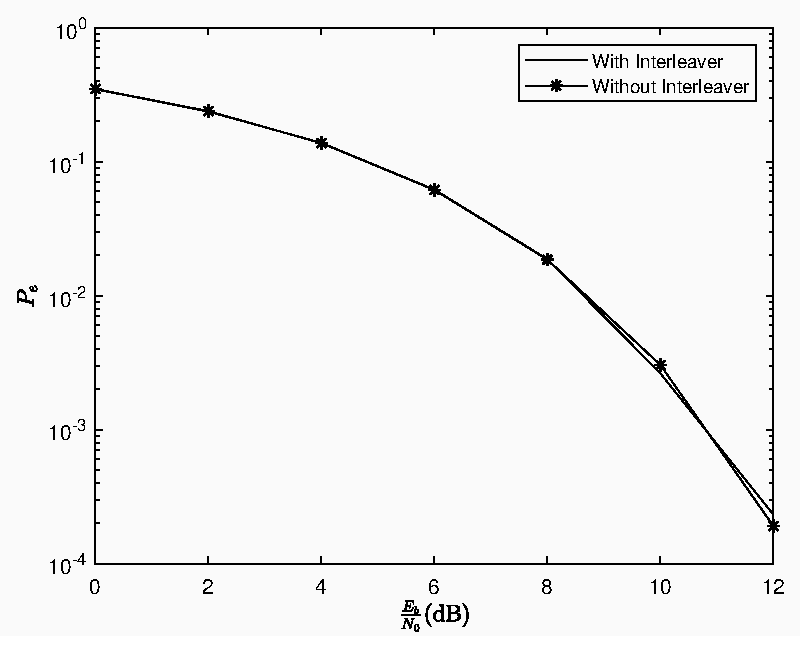
\includegraphics[width=\columnwidth]{./figs/Interleaver.eps}
\end{center}
\caption{Bit interleaver for 8PSK}
\label{fig:inter}
\end{figure}






\section{Physical Layer Framing(PLFRAMING)}

PLFRAMING useful for the specifying modulation scheme and code rate and frame characteristics.In receiver synchronization, Frame synchronization plays a key role. 
%\item In order to form the PLFRAME which is used for receiver synchronization, a header is inserted in the beginning of each frame.



\begin{figure}
\begin{center}
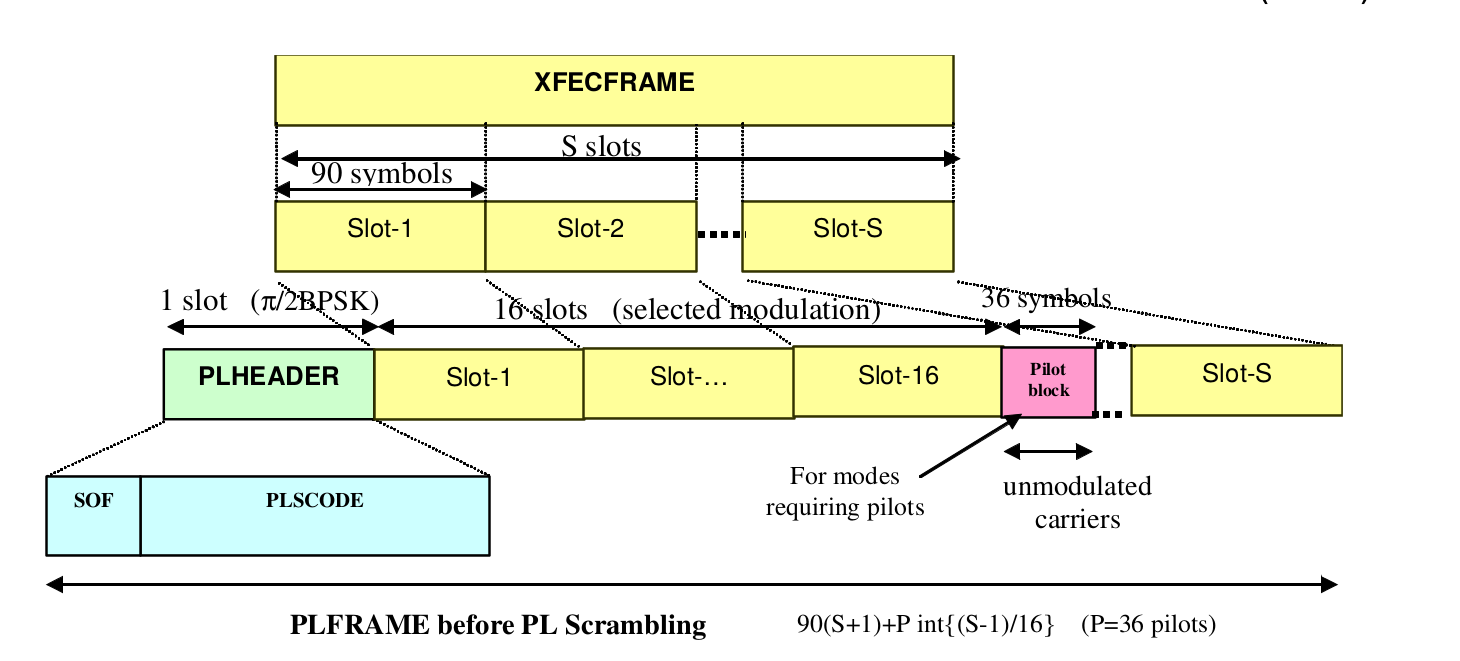
\includegraphics[width=\columnwidth]{/pl_framing}
\end{center}
\caption{Structure of PLFRAME.}
\label{fig:splframe}
\end{figure}

 Fig. \ref{fig:splframe} shows the Typical Structure of PLFRAME according to \cite{dvb}.
 \begin{equation}\label{eq:1}
I_{2i-1}=Q_{2i-1}=\frac{1}{\sqrt{2}}(1-2y_{2i-1}) \quad i=1,2,\dots,45
\end{equation}
\begin{equation}\label{eq:2}
I_{2i}=-Q_{2i}=-\frac{1}{\sqrt{2}}(1-2y_{2i-1}) \quad 1,2\dots,45
\end{equation}
The PLHEADER, represented by binary stream , $y_1,\dots,y_{90}$ is modulated into 90 $\frac{\pi}{2}$-BPSK symbols. Eqs.\eqref{eq:1} and \eqref{eq:2} shows the generation of $\frac{\pi}{2}$-BPSK mapping.


\begin{itemize}
\item PLHEADER consists of two fields,
\begin{enumerate}
\item Starting of Frame(SOF) 26 symbols
\item Physical Layer Signalling Code (PLSC) , 64 symbols
\end{enumerate}
\end{itemize} 
\subsection{Generation of SOF}
SOF consistutes a fixed sequence $18D2E82_{HEX}$ in binary format which is from right to left.
\subsection{Generation of PLSC}
\begin{itemize}
\item Generation of PLSC involes definining 7 symbols and multiplying first 6 symbols with the defined $G$ matrix in \cite{dvb}. First 5 symbols called as MODCOD filed and next 2 symbols as TYPE field.
\item First 5 symbols represents MODCOD which specifies Frame's mapping scheme and code rate.
\item Next 2 symbols represents TYPE filed which specifies Frame length and presence and absesnce of pilot fileds.
(0 = normal: 64 800 bits; 1 = short: 16 200 bits) ; (0 = no pilots, 1 = pilots)
\end{itemize}
%
\begin{figure}
\begin{center}
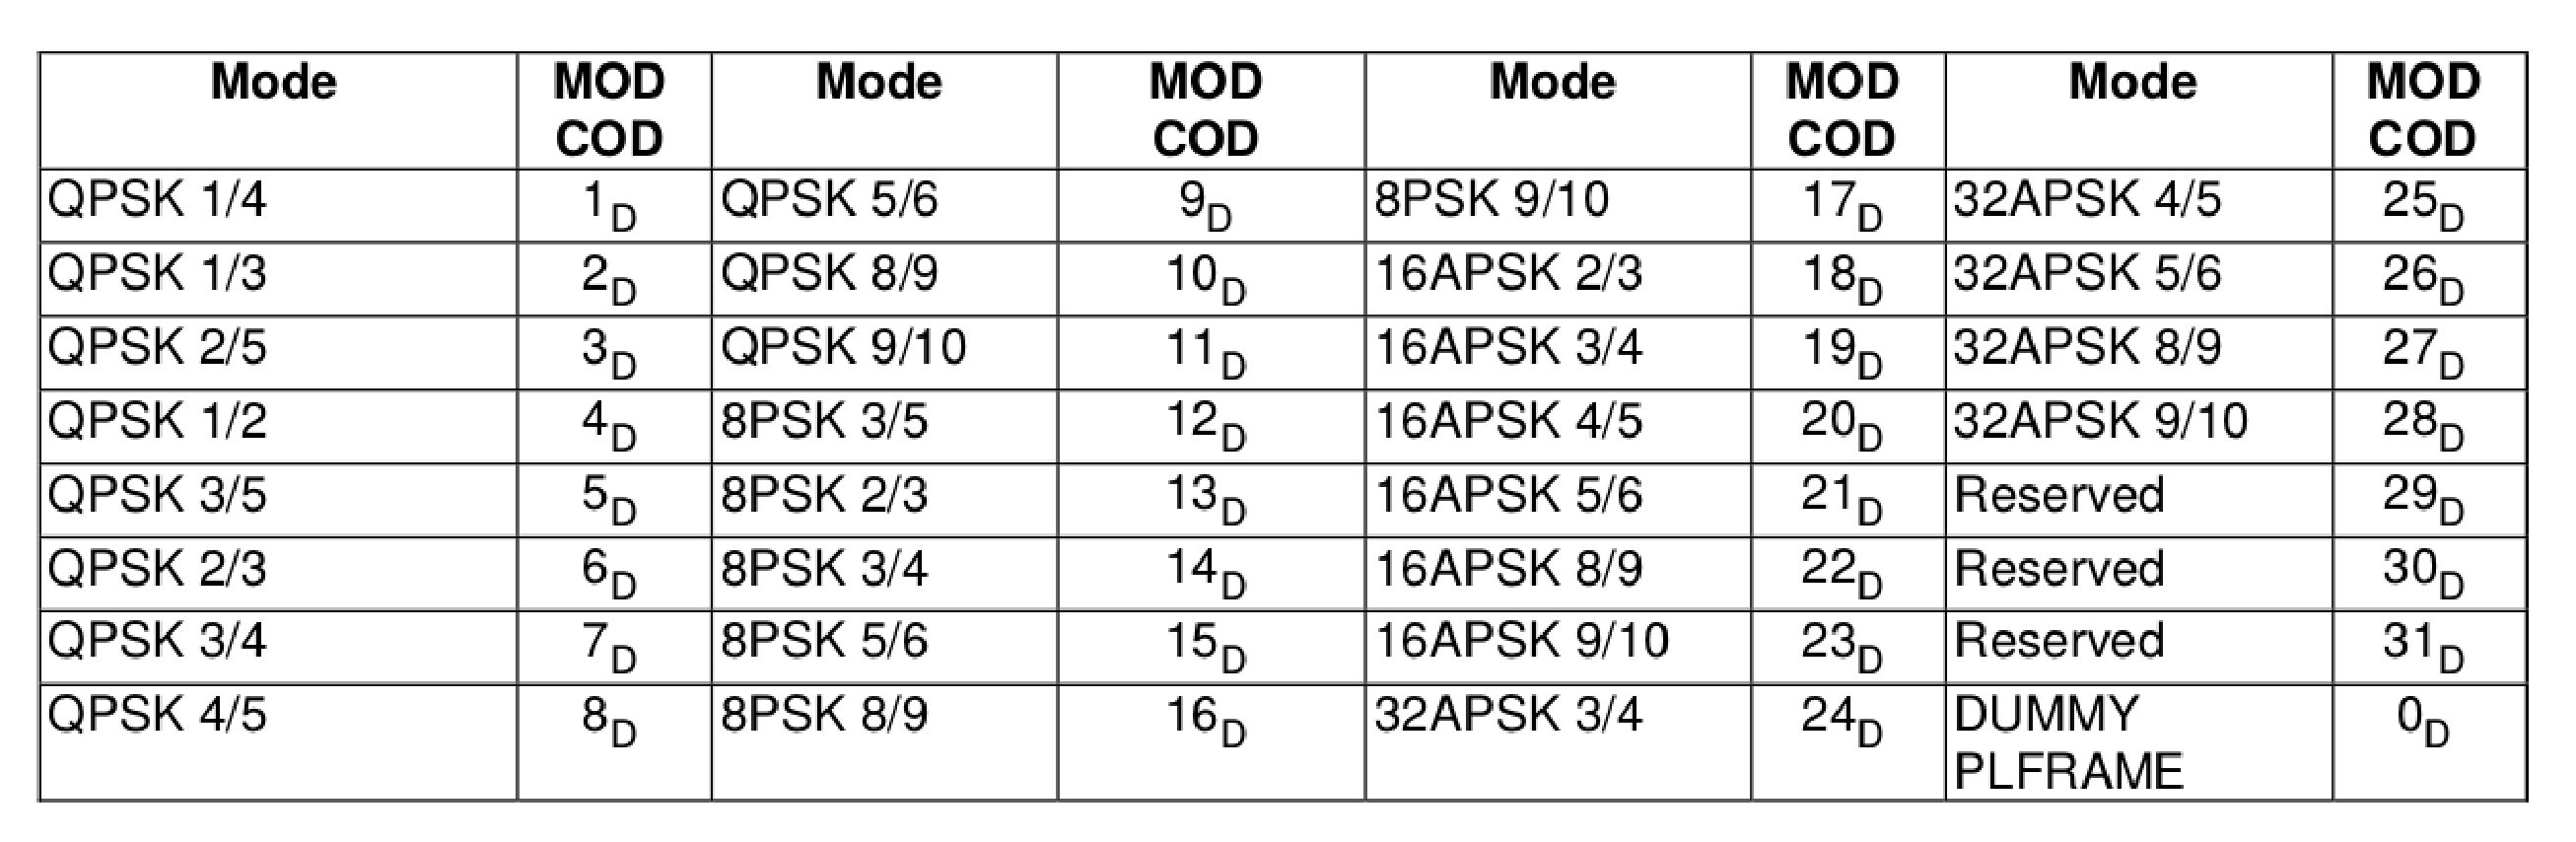
\includegraphics[width=\columnwidth]{/MODCOD}
\end{center}
\caption{MODCOD coding for various mapping schemes}
\label{fig:modcod}
\end{figure}
%
%
\begin{figure}
\begin{center}
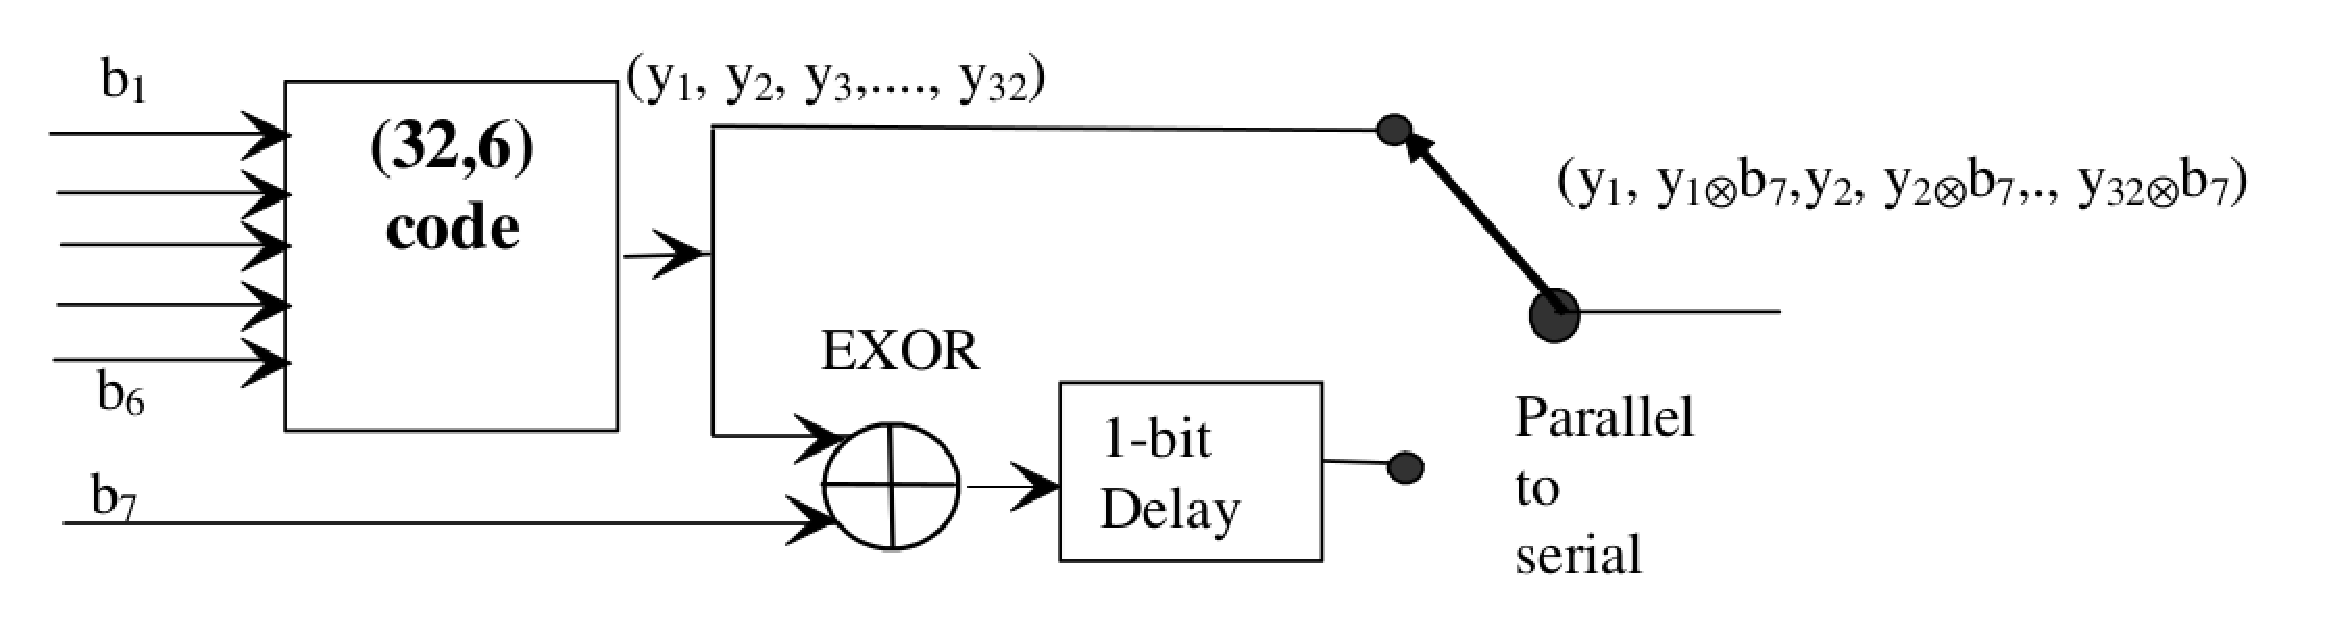
\includegraphics[width=\columnwidth]{/plscode}
\end{center}
\caption{Physical Layer Signalling generation}
\label{fig:pls gen}
\end{figure}
%
 Fig. \ref{fig:modcod} shows the MODCOD coding for various mapping schemes. Similarly, Fig. \ref{fig:pls gen} shows the generation of 64 bits.
 
 After the generation of PLS code, we will again scramble the PLS Code with the fixed SCR sequence which is defined in the \cite{dvb}.
 
\begin{equation}
PLSC=PLSC \oplus SCR
\end{equation}
\subsection{Generation of Pilots}
%
\begin{figure}
\begin{center}
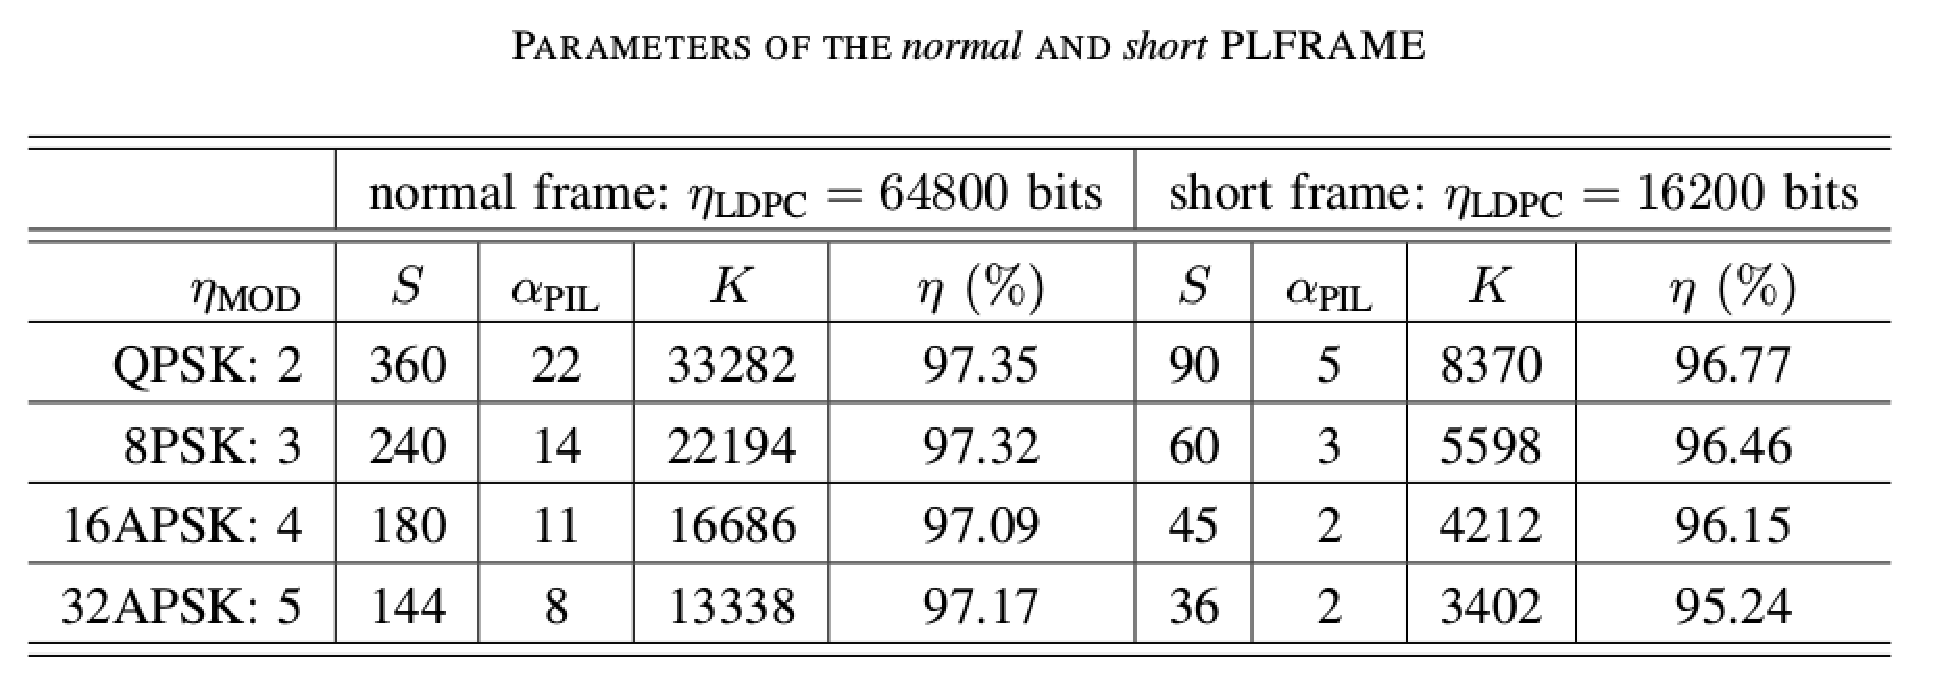
\includegraphics[width=\columnwidth]{/parameters_pl_frame}
\end{center}
\caption{paramters of plframe}
\label{fig:plframe}
\end{figure}
%
Pilot block consists of $P=36$ symbols. Each pilot is composed of un-modulated complex symbol.Where, $I=Q=\frac{1}{\sqrt{2}}$ The first pilot block inserted 16 slots after the PLHEADER and next is inserted after the 32 slots and so on.
\begin{equation}\label{eq:plen}
K = 
\begin{cases}
90\times (S+1)  & \textit{with out pilots}
\\
90\times (S+1) + 36\times \alpha_{PIL}  & \textit{with pilots}
\end{cases}
\end{equation}
Where , $\alpha_{PIL}=\left\lfloor \frac{(S-1)}{16} \right\rfloor$.\\
Eq.\eqref{eq:plen} specifies the total length $K$ of the PLFRAME. Smiliarly, Fig. \ref{fig:plframe} Shows the Parameters of PLFRAME.

% \begin{itemize}
%%\item If pilots are used, then a 36 symbols
%%pilot field is inserted every 16 slots of data symbols. Given that a PLFRAME cannot terminate to a pilot field, the total number of pilot fields is $\alpha_{PIL}=\left\lfloor \frac{(S-1)}{16} \right\rfloor$
%%\item The total length of the PLFRAME in symbols is 
%%\begin{equation}
%%K = 
%%\begin{cases}
%%90\times (S+1)  & \textit{with out pilots}
%%\\
%%90\times (S+1) + 36\times \alpha_{PIL}  & \textit{with pilots}
%%\end{cases}
%%\end{equation}
%%\begin{center}
%%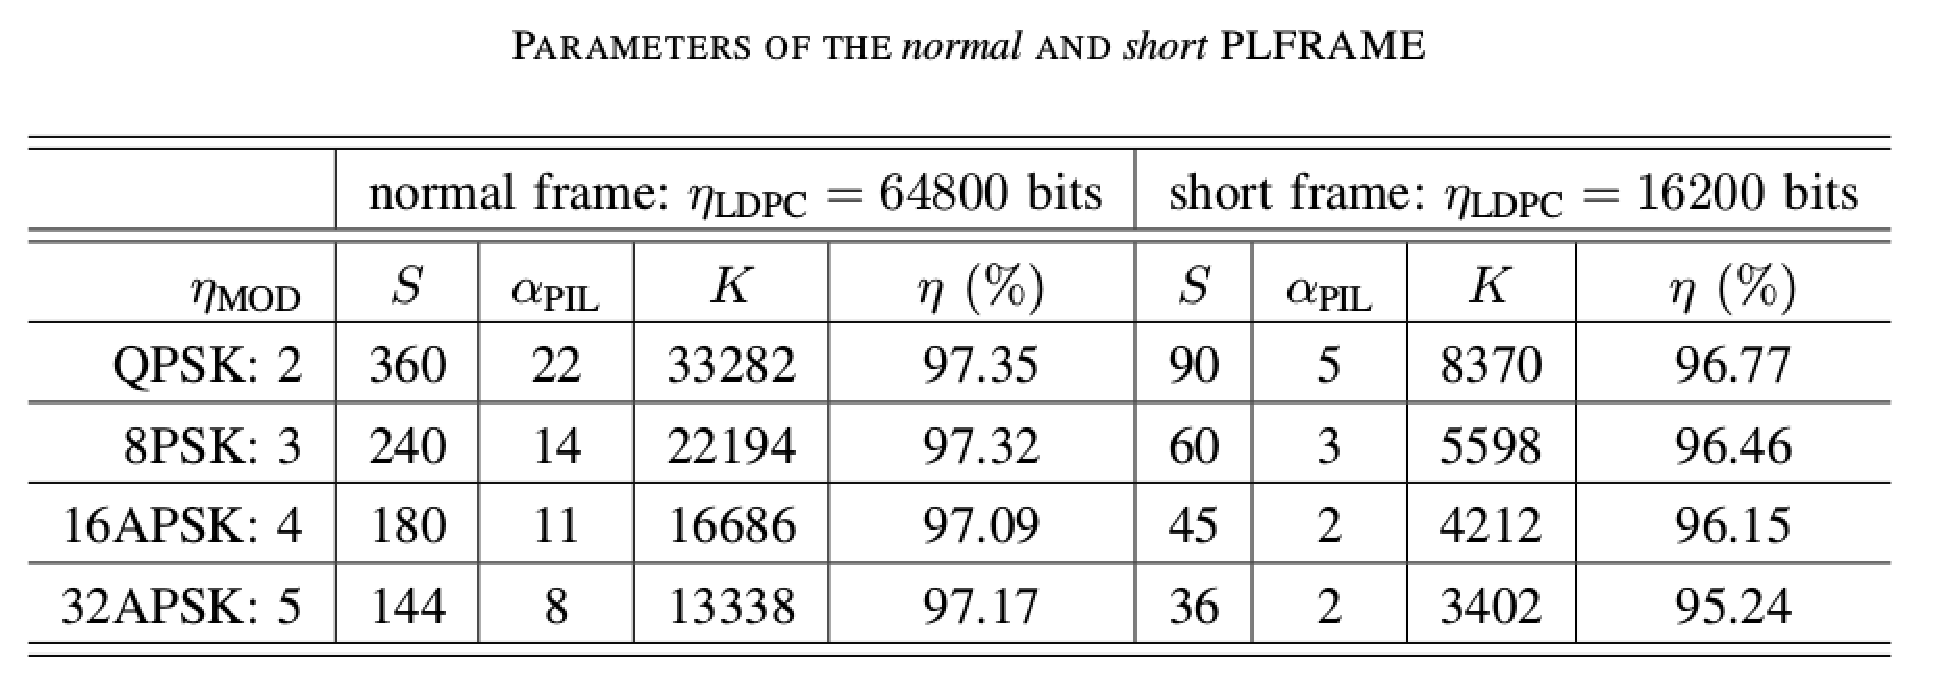
\includegraphics[scale=0.35]{/parameters_pl_frame}
%%\end{center} 
%
%\item The different frame formats,parameters of the normal andshort DVB-S2 frame for all constellation formats were tabulated in above table as  specified in \cite{dvb}
%\end{itemize}

\section{Pulse Shaping}
\begin{equation}
Y_k(m)=H_k(m) \ast X_k + V_k(m) \quad m=1,\dots, M; k=1,\dots,N
\end{equation}
Where,$H_k$ represents the pulse shape,$V_k(m) \sim \mathcal{N}\brak{0,\sigma^2} $.

At the Receiver we will,
\begin{align}
Y_k(m)\ast H^*_k(M-m) =H^*_k(M-m)\ast H_k(m) \ast X_k + V_k(m) 
\end{align}

$H(f)$ will be choosen from the \cite{dvb} which is converted to time domain form to get $ H_k(m)$
\begin{align}
H(f) =\begin{cases}
1& \abs{f}<f_N(1-\alpha)\\
\cbrak{\frac{1}{2}+\frac{1}{2}\sin \frac{\pi}{2}\sbrak{\frac{f_N-\abs{f}}{\alpha}}}^{\frac{1}{2}}&\abs{f}=f_N(1-\alpha)\\
0&\abs{f}>f_N(1-\alpha)
\end{cases}
\end{align}
%\begin{itemize}
%\item After randomization, the signals shall be square root raised cosine filtered. The roll-off factor shall be $\alpha$ = 0,35, 0,25and 0,20, depending on the service requirements.
%\item Suitable $H(f)$ will be choosen from the \cite{dvb}.
%\begin{align}
%H(f) =\begin{cases}
%1& \abs{f}<f_N(1-\alpha)\\
%\cbrak{\frac{1}{2}+\frac{1}{2}\sin \frac{\pi}{2}\sbrak{\frac{f_N-\abs{f}}{\alpha}}}^{\frac{1}{2}}&\abs{f}=f_N(1-\alpha)\\
%0&\abs{f}>f_N(1-\alpha)
%\end{cases}
%\end{align}
%
%\end{itemize}

\bibliography{IEEEabrv,others.bib}
\end{document}

